\begin{figure}[!h]
	\centering
	\subbottom[satellite image\label{fig:egsatellite}]
		{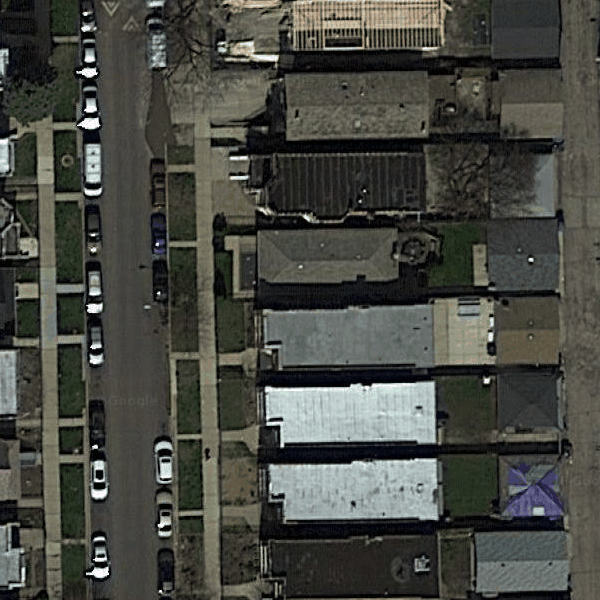
\includegraphics[width=0.328\textwidth]{4-00-0.png}}
	\subbottom[roadmap image\label{fig:egroadmap}]
		{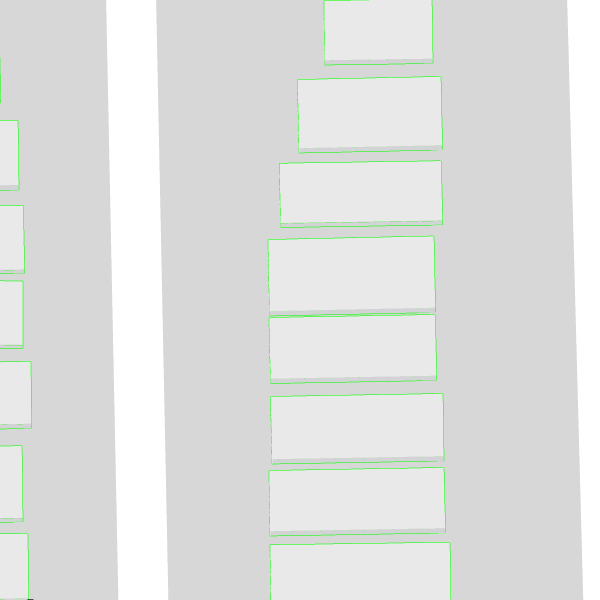
\includegraphics[width=0.328\textwidth]{4-00-1.png}}
	\subbottom[hybrid image\label{fig:eghybrid}]
		{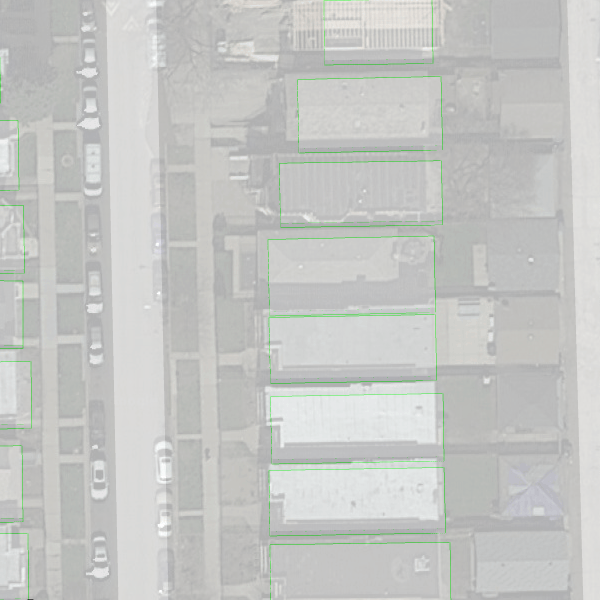
\includegraphics[width=0.328\textwidth]{4-00-2.png}}
    \caption{Example images downloaded through Google Static Maps API. (a) and (b) are obtained directly by the API, with 41.9399708 degrees north latitude, 87.7380649 degrees west longitude of the center (located in Chicago), both width and height 600 pixels, zoom level 20 and scale 1, but different in map types. (c) is obtained by overlaying (a) with (b), with 75\% opacity. It can be clearly seen that the two images cannot match very well.}
	\label{fig:egapimap}
\end{figure}